\chapter{Entrepreneurs: An Interesting Perspective on Building Wealth}

This interview is brief, but its structure is unusually tight. We begin with a career question asked from the standpoint of an engineer, we receive an answer before we receive its proof, and then the proof is supplied by a few large quantitative facts: the present scale of the world economy, its present dependence on fossil fuels, its projected growth by 2050, and the added requirement of net zero. The mathematics is modest, but the logic is not. The claim is that wealth will be created where an enormous system must both expand and transform.

\section{Opening Setup}

The interviewer does not ask for an abstract philosophy of money. He asks what industry one should pursue, then identifies himself as an engineer, and only then sharpens the issue: how does someone become wealthy in 2022? We should preserve that order, because it tells us how to hear the answer. The issue is not merely where capital may earn a return. It is where a technically trained builder should go.

What follows is therefore a directional argument. We are not given a menu of sectors. We are given a single sector-level thesis and then a compact explanation of why that thesis is plausible.

\section{The Wealth Question}

The decisive stylistic move of the clip is that the answer arrives immediately. The speaker does not begin with a long preamble. He places a flag in the ground and then works backward to the supporting quantities.

\subsection{Question \& Answer}

The question is plain: how can someone become wealthy in 2022? The answer is equally plain: the next 1{,}000 unicorns will be in green tech.

This is the right place to pause. A sentence like this can easily be mistaken for a slogan. But in the interview it is not offered as a slogan. It is offered as a compressed conclusion that will immediately be justified by scale, dependence, growth, and constraint. We should therefore read it as the final line of an argument that is about to be unpacked, not as free-floating enthusiasm.

\section{The Present Baseline}

The justification begins with the present world. Let us introduce a small amount of notation, explicitly as editorial shorthand for the spoken claims.

\begin{definition}
Let \(W_t\) denote the scale of the world economy at year \(t\), let \(f_{\mathrm{fossil},t}\) denote the rough share of the system that depends on fossil fuels, and let \(E_{\mathrm{net},t}\) denote the net-emissions condition. These symbols are not quoted board notation; they are a compact way to preserve the interview's quantitative logic.
\end{definition}

The first baseline number is the scale of the present economy:
\begin{equation}
W_{2022} \approx \$90\text{ trillion}.
\end{equation}
The second baseline number is the claimed dependence on fossil fuels:
\begin{equation}
f_{\mathrm{fossil},2022} \approx 0.8.
\end{equation}

What matters here is not fine statistical interpretation. The speaker is not offering a sector-by-sector accounting. He is saying that the current productive system is already enormous, and that most of it still rests on a fossil-fuel base. This gives the argument a large starting mass. The transition, if it comes, is not a side project attached to a small niche economy. It acts on the main body of the world system.

\begin{remark}
The \(80\%\) figure should be handled cautiously. In the interview it functions as a rough indicator of fossil dependence, not as a carefully defined variable tied to one precise denominator. We use it here only to preserve the order-of-magnitude claim.
\end{remark}

\section{The 2050 Shift}

The next move is temporal. Having fixed the size and structure of the present system, the speaker jumps to 2050 and adds a second condition. The future economy is not merely cleaner. It is also bigger.

The time horizon is stated explicitly:
\begin{equation}
2050 - 2022 = 28.
\end{equation}
Over this horizon the world economy is said to double:
\begin{align}
W_{2050} &\approx 2W_{2022},\\
W_{2050} &\approx \$180\text{ trillion}.
\end{align}
At the same time, the future system is required to satisfy a net-zero condition:
\begin{equation}
E_{\mathrm{net},2050} \approx 0.
\end{equation}

This is the hinge of the whole argument. If the future were merely net zero with no growth, we would face one kind of replacement problem. If the future were merely larger with no carbon constraint, we would face a different kind of expansion problem. The interview fuses the two. The world must build a larger productive base while abandoning the dominant energetic basis of the current one.

\begin{figure}
\centering
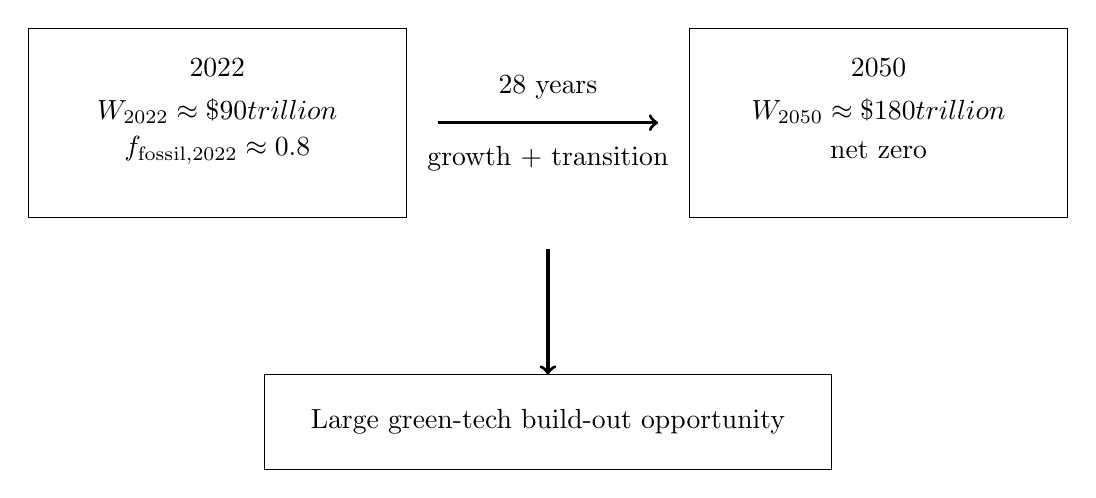
\begin{tikzpicture}[x=1cm,y=1cm]
\draw (0,0) rectangle (4.8,2.4);
\node at (2.4,1.9) {2022};
\node at (2.4,1.35) {$W_{2022}\approx \$90\text{ trillion}$};
\node at (2.4,0.85) {$f_{\mathrm{fossil},2022}\approx 0.8$};

\draw[->, very thick] (5.2,1.2) -- (8.0,1.2);
\node at (6.6,1.65) {$28$ years};
\node at (6.6,0.75) {growth + transition};

\draw (8.4,0) rectangle (13.2,2.4);
\node at (10.8,1.9) {2050};
\node at (10.8,1.35) {$W_{2050}\approx \$180\text{ trillion}$};
\node at (10.8,0.85) {net zero};

\draw[->, very thick] (6.6,-0.4) -- (6.6,-2.0);
\draw (3.0,-3.2) rectangle (10.2,-2.0);
\node at (6.6,-2.6) {Large green-tech build-out opportunity};
\end{tikzpicture}
\end{figure}

The figure is not a reconstruction of a visible board. It is an editorial diagram of the transcript's internal logic: present scale, future scale, and the net-zero constraint converge to produce a large entrepreneurial search space.

\section{A Worked Transition Estimate}

We can now extract the interview's arithmetic without pretending that the interview supplied a formal model. A useful way to proceed is to turn the spoken numbers into an order-of-magnitude estimate.

\paragraph{Step 1: Estimate the fossil-linked portion of the present system.}

If we take the spoken \(80\%\) at face value as a rough multiplier, then the part of the current world economy tied to fossil fuels is approximately
\begin{align}
W_{\mathrm{fossil\text{-}linked},2022}
&\approx f_{\mathrm{fossil},2022}W_{2022}\\
&\approx 0.8 \times \$90\text{ trillion}\\
&\approx \$72\text{ trillion}.
\end{align}

\paragraph{Step 2: Estimate the added scale of the future economy.}

The interview also gives us a rough increment in total output:
\begin{align}
\Delta W
&\approx W_{2050} - W_{2022}\\
&\approx \$180\text{ trillion} - \$90\text{ trillion}\\
&\approx \$90\text{ trillion}.
\end{align}

\paragraph{Step 3: Read the two requirements together.}

The point is not that \(\$72\) trillion and \(\$90\) trillion can simply be added as clean accounting categories; they cannot. The point is that, at the scale of the speaker's own numbers, we are dealing simultaneously with
\begin{enumerate}
\item a vast installed productive base that is still fossil-linked, and
\item a further vast increment of growth that must arrive under a net-zero condition.
\end{enumerate}

So the transition problem can be summarized schematically as
\begin{equation}
\bigl(W_{2050} \approx 2W_{2022}\bigr)
\land
\bigl(f_{\mathrm{fossil},2022} \approx 0.8\bigr)
\land
\bigl(E_{\mathrm{net},2050} \approx 0\bigr)
\Rightarrow
\text{large green-tech build-out opportunity}.
\end{equation}

This is not a theorem. It is a disciplined restatement of the speaker's mechanism. Wealth appears where a civilization-sized coordination problem requires new energy systems, new infrastructure, new software, new financing structures, and new industrial methods.

\section{Why This Points to Green Tech}

We can now see why the answer comes before the proof. Once the scale-and-constraint structure is laid out, the forecast about green tech is no longer arbitrary. The claim is that the next generation of very large firms will emerge where the world has no choice but to rebuild.

In that sense, the phrase ``the next 1{,}000 unicorns'' is not functioning as a measured output of a model. It is functioning as a way to name the entrepreneurial surface area created by transition. If a technical founder asks where effort is most leveraged, the answer given here is: go where a huge fossil-dependent system must be made compatible with a much larger net-zero future.

The emphasis on engineering at the start now returns with full force. The argument is not primarily about passive allocation into an already mature asset class. It is about design, construction, deployment, and replacement at scale. Green tech is ``the place to go'' because it sits exactly where technical difficulty and economic necessity coincide.

\section{Summary}

The lecture is short, but its structure is clean. We begin with a practical question from an engineer. We are then given a sharp answer: green tech. The answer is defended by four quantities or conditions: a \(\$90\) trillion present world economy, rough \(80\%\) fossil dependence, a doubling to \(\$180\) trillion by 2050, and a net-zero endpoint. From these, the speaker infers an enormous build-out problem.

That is the mathematical spine of the chapter. It is not a detailed climate model, nor a full theory of firm formation. It is a scale argument. When a system this large must both grow and transform, the search for wealth moves toward the industries that make the transformation possible. Green tech is presented as the most consequential instance of that rule.